\documentclass{article} % For LaTeX2e
\usepackage{nips14submit_e,times}
\usepackage{hyperref}
\usepackage{url}
\usepackage{graphicx}
\usepackage[super]{nth}
\usepackage{todonotes}
\usepackage{amsfonts}

%\documentstyle[nips14submit_09,times,art10]{article} % For LaTeX 2.09

\title{CPSC 536N Project: Gossip Protocols with Random Linear Network Coding}
\author{
Neil~Newman\\
81435142\\
Department of Computer Science\\
University of British Columbia\\
Vancouver, BC V6T 1Z4 \\
\texttt{newmanne@cs.ubc.ca}
}
\newcommand{\fix}{\marginpar{FIX}}
\newcommand{\new}{\marginpar{NEW}}

\def\numNodes{\textit{n}\,}
\def\graph{\textit{G(t)}\,}
\def\graphtime{\textit{t}\,}
\def\numMessages{\textit{k}\,}
\def\RLNC{\textit{RLNC}\,}
\def\fieldSize{\textit{q}\,}
\def\dualSpace{$Y_u^{\perp}$\,}
\def\field{\mathbb{F}_{\fieldSize}\,}


\nipsfinalcopy % Uncomment for camera-ready version

\begin{document}

\maketitle

\section{Introduction}
\paragraph{Gossip Protocols}
Gossip protocols are randomized algorithms used to spread information within a network. Initially, some set of messages are scattered throughout the network (each node may know none, some, or all of the messages), and the goal is to make every node in the network know all of the messages. Gossip protocols are modeled on the way that rumours spread among a society or the way in which a disease outbreak spreads throughout a population (gossip protocols are sometimes referred to as epidemic alogrithms). The protocol achieves this through a series of rounds in which nodes exchange messages in random pairwise interactions. The message that a node chooses to send is never conditioned on who the receiver will be: the sender does not know what the receiver does or does not know, and it would be too expensive to query this information or for the sender to sned all of the messages it knows about.

\paragraph{Why Gossip Protocols?}
Like many other randomized algorithms, gossip protocols are very simple both from an implementation persepective and to reason about their eventual correctness. In spite of their simplicity, gossip protocols are well suited to a wide variety of network types, including dynamic networks, very large networks, and unreliable networks. In contrast to some non-randomized algorithms used to spread information through a network (for example, anything that would require constructing a spanning tree) gossip algorithms do not take the structure of the network into account. This fact makes gossip protocols suitable for use in real networks, in which communication links can fail, and nodes and can enter and leave the network at any time. 

\paragraph{Random Linear Network Coding}
One issue with gossip protocols is that if the goal is to spread multiple messages in parallel, a node need to choose which information it sends in each interaction without knowledge of what the other node knows or does not know (acquiring this knowledge would be expensive, as would be sending all of the information that it knows). If the node were to simply choose a random message that it knew about, it is possible for some messages to become widely spread while others remain rare, so that the stopping time for the algorithm, (the point at which every node knows all of the messages) could be dominated by the time it takes to propogate the rare messages. This can be circumvented by using gossip protocol based on \emph{Random Linear Network Coding} (RLNC). In this protocol, discussed in more detail in \ref{subsec:RLNC}, a node sends a message that is a random linear combination of the messages that it knows. The original messages can be recovered using Gaussian elimination once a node has received enough linearly independent coefficient vectors--however, it should be noted that until this time, it is possible that the node will not be able to decode any of the individual messages (i.e. it can be all or nothing). The additional overhead of the coefficients on the packets sent is quite low if the messages are long and the number of total messages is significantly less than the message length.

\paragraph{When to stop: Hot rumours}
A problem in gossip protocols is to know when the protocol can safely be terminated. In some applications, it may not make sense to run the protocol indefinitely. A node chooses another node at random and performs a complete exchange of knowledge. This is prohibitively expensive, but can be used occasionally to guarantee eventual consistency. Rumor mongering is another method of distributing information. When a node receives a message, the message is a \textit{hot rumor}. As long as the rumor is hot, the node will periodically connect with another random node and see if it knows about the rumor. If the node tries to share a rumor and the other node already knows about it, then the rumor cools off. Eventually, the node stops propagating the rumor entirely. 

\paragraph{This paper}
The goals of this paper are as follows: Firstly, to summarize the results and techniques used to prove bounds on the expected stopping times of gossip protocols based on RLNC in \cite{haeupler2011analyzing}. Secondly, to verify these results experimentally and compare the RLNC gossip algorithm to other variants of gossip protocols. 

\paragraph{Applications}
Gossip protocols can be applied to database replication as demonstrated in \cite{demers1987epidemic}, which describes gossip protocol used to share updates with other database nodes deployed successfully at Xerox PARC. Cassandara  \cite{lakshman2010cassandra}, a popular distributed database management system, uses a gossip protocol in which nodes share their state information and information about a few other nodes that they know about with other nodes allowing each node to quickly build up a global picture of the network without any centralization. \cite{export:67453} describes Avalance, a bittorrent alternative which removes the problem of thinking about how to schedule what blocks to download by using RLNC.

\subsection{Model of Network and Communication}
We will use the model from \cite{haeupler2011analyzing}, which is as follows: There are \numNodes nodes in the network. A network is a graph \graph that can be static ($\graph = G  \forall \graphtime$) or can vary with time \graphtime and is either directed or undirected. An edge in \graph from any two nodes \textit{a} and \textit{b} represents a link through which communication can take place in round \graphtime; if the edge is directed it means that communication can only occur in the direction of the edge. There are \numMessages distributed over the network (see \ref{subsec:startingconditions} for details on the ways in which we consider the messages to be distributed).  

\subsection{RLNC Algorithm}\label{subsec:RLNC}
\paragraph{Preliminaries}
Packets are vectors over a finite field $\mathbb{F}_{\fieldSize}$, where the size of the field, \fieldSize, is a prime or prime power. Addition and mulitplication in the remainder of this description are over $\mathbb{F}_{\fieldSize}$. There are \numMessages messages, $\vec{m_{1}}...\vec{m_{\numMessages}}$ that are vectors from $\mathbb{F}_{\fieldSize}^{l}$. Packets are of the form ($\vec{\mu}, \vec{m}$), where $\vec{m} = \sum_{i=1}^{\numMessages} \mu_i\vec{m_i} \in \mathbb{F}_{\fieldSize}^{l}$ and $\vec{\mu} = (\mu_1,...,\mu_k) \in \mathbb{F}_{\fieldSize}^{\numMessages}$ is the coefficient vector. Note that if a node ever knows enough coefficient vectors such that the span of these vectors equals $\mathbb{F}_{\fieldSize}^{\numMessages}$ then Gaussian elimination can be used to reconstruct all of the messages. Therefore, a minimum of \numMessages packets with linearly independent coefficients are needed. The choice of \fieldSize is a trade-off between the size of messages in bytes (because of the space needed to store the coefficients) and the convergence rate; we use $\fieldSize=2$ for the remainder of this paper. 
\paragraph{Algorithm}
Every node \textit{v} keeps a subspace $X_v$ that is the span of all of the packets it currently knows. When a packet needs to be chosen to send, a node chooses a packet uniformly at random from $X_v$. When a packet is received, $X_v$ is recomputed. If $X_v = \mathbb{F}_{\fieldSize}^{\numMessages}$ then a node can decode messages. When this is true for every node, the algorithm is considered to have stopped. 
\paragraph{Practical Details}
Every node maintains only messages that are \textit{helpful}, that is, messages that increase the rank of the coefficient matrix: a matrix in which every row corresponds to a previously received message's coefficients. We refer to the subspace spanned by these coefficients as $Y_v$. If a node begins knowing a particular message, say message $i$, then it's coefficient matrix is initialized to begin with the $ith$ standard basis vector. To determine whether or not a new message contains helpful coefficients, we compute the rank of the current matrix and the rank of the current matrix with an additional row for the new message's coefficients. If the rank has increased, the message is helpful and we add it to the node's collection of messages (and its coefficients to the coefficient matrix). Otherwise, the message provided no new information, and so it is ignored. When the rank of the coefficient matrix is equal to the number of messages, a node can decode all of the messages. When this condition is true for every node, we say that the algorithm has terminated. In order to send out a random message, a node generates a uniformly random coefficient in $\mathbb{F}_{\fieldSize}$ for message it knows, and then sends out the linear combination of its known messages and these coefficients.

\subsection{Modes of communication}\label{subsec:communication}
We allow the following four modes of communication:
\begin{itemize}
\item \texttt{BROADCAST} A node sends to all of its neighbours
\item \texttt{PUSH} A node sends to one neighbour chosen uniformly at random
\item \texttt{PULL} A node chooses a neighbour uniformly at random and receives a message from the neighbour
\item \texttt{EXCHANGE} A node chooses a neighbour uniformly at random and they each send each send each other a message
\end{itemize}
The choice of what packet to send is never conditioned on the who will receive the packet.

\subsection{Timing models}
We consider synchronous models in which every node in the network can send a message once per round. Asynchronous models have also been studied in the literature.

\subsection{Starting conditions}\label{subsec:startingconditions}
We consider the following starting conditions:
\begin{itemize}
\item \texttt{DISTRIBUTED} Each node knows a single, unique message
\item \texttt{SINGLE} A single node knows every message, other nodes know nothing
\end{itemize}

\subsection{Graph types}
\begin{itemize}
\item \texttt{COMPLETE} Every node is connected to every other node
\item \texttt{ADVERSARIAL} An adversary gets to choose the set of edges at every time \graphtime (subject to the constraint that \graph must remain connected). For example, if there is only a single message to distribute, an adversary might choose to only put a single link between the set of nodes that know the message and the set of nodes that don't know the message. 
\end{itemize}

\subsection{Proof techniques and summary of theoretical results}
\paragraph{Proof techniques}
If an algorithm achieves a stopping time of $O(\numMessages + T)$, where $T$ is the time that it takes to distribute a single message amongst all of the nodes, then it is said to achieve perfect pipelining, because the startup cost is paid only once, and every subsequent message does not need to pay the startup cost.
\cite{deb2006algebraic} shows that the probability that a node sends a helpful message (one that increases the rank of the coefficient matrix) is at least $1 - 1/\fieldSize$, provided that it was possible for the node to send a helpful message (i.e. if node $v$ sends a message to node $u$, and $Y_v \subseteq Y_u$, then no helpful message is possible to send). 
\cite{haeupler2011analyzing} looks at how the orthogonal complement of $Y_u$, \dualSpace, shrinks monotonically to the empty span. Note that because we are operating in a field, the dot-product is not positive definite and so the concept of orthogonal does not match geometrical intuition. They pick a fixed vector in \dualSpace and determine how long it takes before it dissapears from $Y_u$ with high probability. Then a union bound is taken over every one of the $\fieldSize^{\numMessages}$ vectors in \dualSpace. The spreading is a monotone Markov process, which has an exponentially decaying tail. 

A node knows about $\vec{\mu} \in \field$ if its coefficient subspace $Y_u$ is not orthogonal to $\vec{\mu}$ ($\exists \vec{c} \in Y_u s.t. < \vec{c}, \vec{\mu}) > \neq 0$). Knowledge about a particular $\vec{\mu}$ spreads with probability $1 - 1/\fieldSize$. Over all the nodes, knowledge of a fixed vector is a monotone increasing set growing process that is a monotone Markov process and therefore has an exponentially decaying tail. 

Choose a $\delta > 0$. Imagine that in some network, a node $v$ is trying to disseminate one single message. It does this in the following way: every round, every node that knows the message broadcasts to all of its neighbours with probability $1 - 1/\fieldSize$. If, for every choice of $v$ in the network, the probability that the message is successfully spread after \graphtime rounds is at least $1-\delta\fieldSize^{-\numMessages}$, then \numMessages messages could be spread in the same network in time \graphtime with probability $1-\delta$ using RLNC gossip with a field size \fieldSize. This is because is a node $u$ sends a message to node $v$ and $u$ knows $\vec{\mu}$, then $v$ will now know $\vec{\mu}$ with probability $1-1/\fieldSize$. This is equivalent to the faulty broadcasting system described above. We assumed that after \graphtime steps, the probability for any given vector that it failed to spread is at most $\delta\fieldSize^{-\numMessages}$, so taking a union bound over all $\fieldSize^{\numMessages}$ vectors gives a probability that after \graphtime rounds all nodes know about all vectors with probability at least $1-\delta$.

The trick then becomes to model the time it takes to disseminate a single vector in the faulty broadcast model. Define a successful round such that at most $T$ successful rounds are needed to spread the vector, and the round is not a success with at most probability $p$. The exact definition will depend on the network properties (expansion, cuts, diamater etc.) and will determine how many nodes need to learn about the vector in a successful round.  
\paragraph{Complete graphs - The Random Phone Call Model}
The random phone call model is a model where \graph is the complete graph. At each time \graphtime, every node randomly phones another node and either PUSH, PULL, or EXCHANGE communication takes place.  In a complete graph, RLNC gossip achieves perfect pipelining, and $T$ is $\Theta(\log{n})$ with high probability. 
Proof: A node has an $1/(\numNodes-1)$ chance of being dialed by another node, and since this true for all $\numNodes-1$ nodes, a node receives in expectation $\Theta(1)$ packets in a round. If even a single node does not know any messages at the start, the algorithm must run for at least $\Omega(\numMessages)$ rounds. Imagining that a single node tries to spread a single message, it will take at least $\Omega(\log{n})$ time to spread it to all nodes (in the best case, after the first round, 1 node knows the message, then 2 nodes after the second, then 4 nodes after the third etc.). Therefore, this model is $\Omega(\numMessages + \log{n})$. To show that it is also $\O(\numMessages + \log{n})$, fix a coefficient vector $\vec{\mu}$ and label a succesful round as one in which the number of nodes that know about $\vec{\mu}$ increases by a constant factor, $\lambda > 1$. Because of this constant factor, it will take at most $O(\log{n})$ rounds until every node knows about $\vec{\mu}$. To complete the proof, they show that a successful round occurs with constant probability. We will summarize the proof for the PULL model. At first, $i < \numNodes/2$ nodes know about $\vec{\mu}$ and therefore at least $\numNodes/2$ nodes are trying to pull $\vec{\mu}$. Each individual node will pull from a node that knows $\vec{\mu}$ with probability $i/\numNodes$, and therefore in expectation at least $i/2$ nodes will receive a message from a node that knows $\vec{\mu}$. With a fixed \fieldSize, after such a pull the node will know $\vec{\mu}$ with probability $1-1/\fieldSize$.  Therefore, at least $\Omega(i)$ nodes learn $\vec{\mu}$ with constant probability each round. 

A later result in the paper shows that in the random phone call model with the PULL type communication, $k>\log{n}^{1+o(1)}$ messages can be spread in $k(1+o(1))$ time if a each message is initially known to a unique node.

Describe the one more thing you will actually experiment on: 

Summarize other key resuls very quickly and proof techniques used:
\paragraph{title}
\paragraph{Random Networks}
Many proofs rely on connectivity properties of \graph that have to hold for every time \graphtime. We can also consider the union of graphs over multiple rounds, $G'(t) = G(3t') \cup G(3t'+1) \cup G(3t'+2)$.


\subsection{Practical details}
Experiments were performed using \textit{python} and \textit{sage}. The \textit{networkx} library was used to generate graphs.

\subsection{Results}
\begin{figure}
\centering
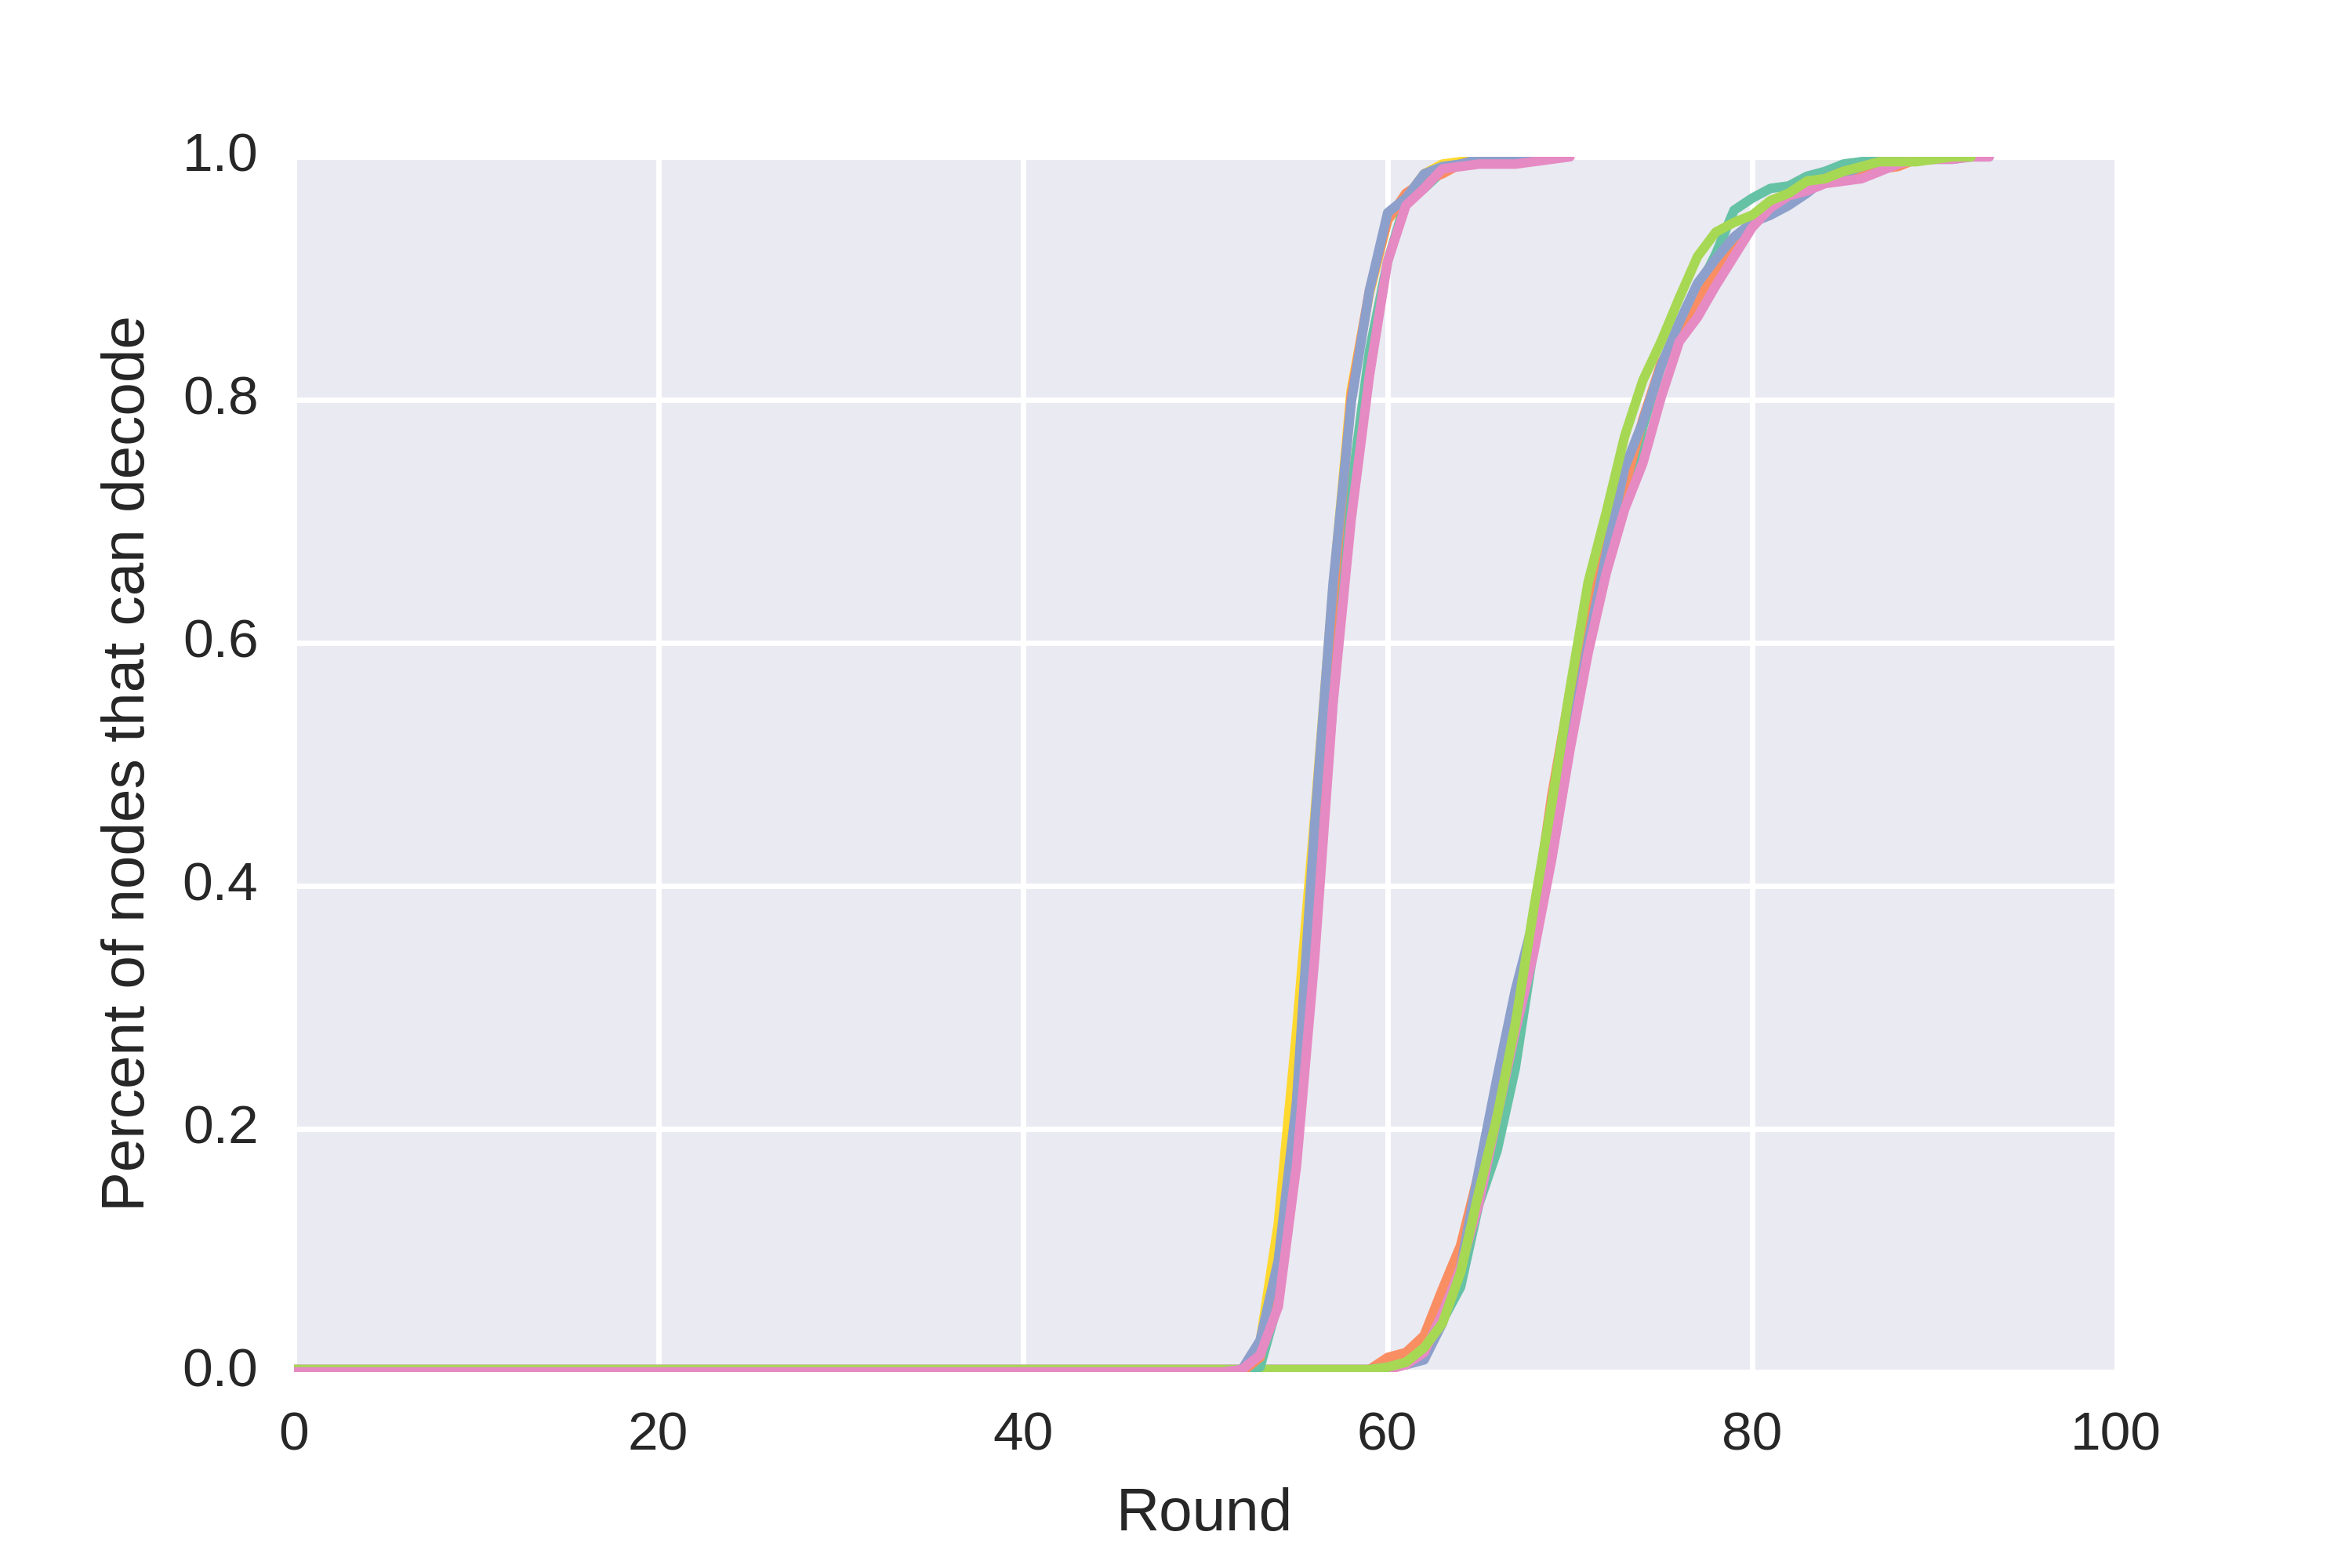
\includegraphics[width=\linewidth]{figures/rlnc-ecdf.png}
\caption{Cumulative distribution showing what fraction of nodes can decode the messages at any given round. 5 trials were performed using 500 nodes and 50 messages.}
\label{fig:rlnc-ecdf}
\end{figure} 
\begin{figure}
\centering
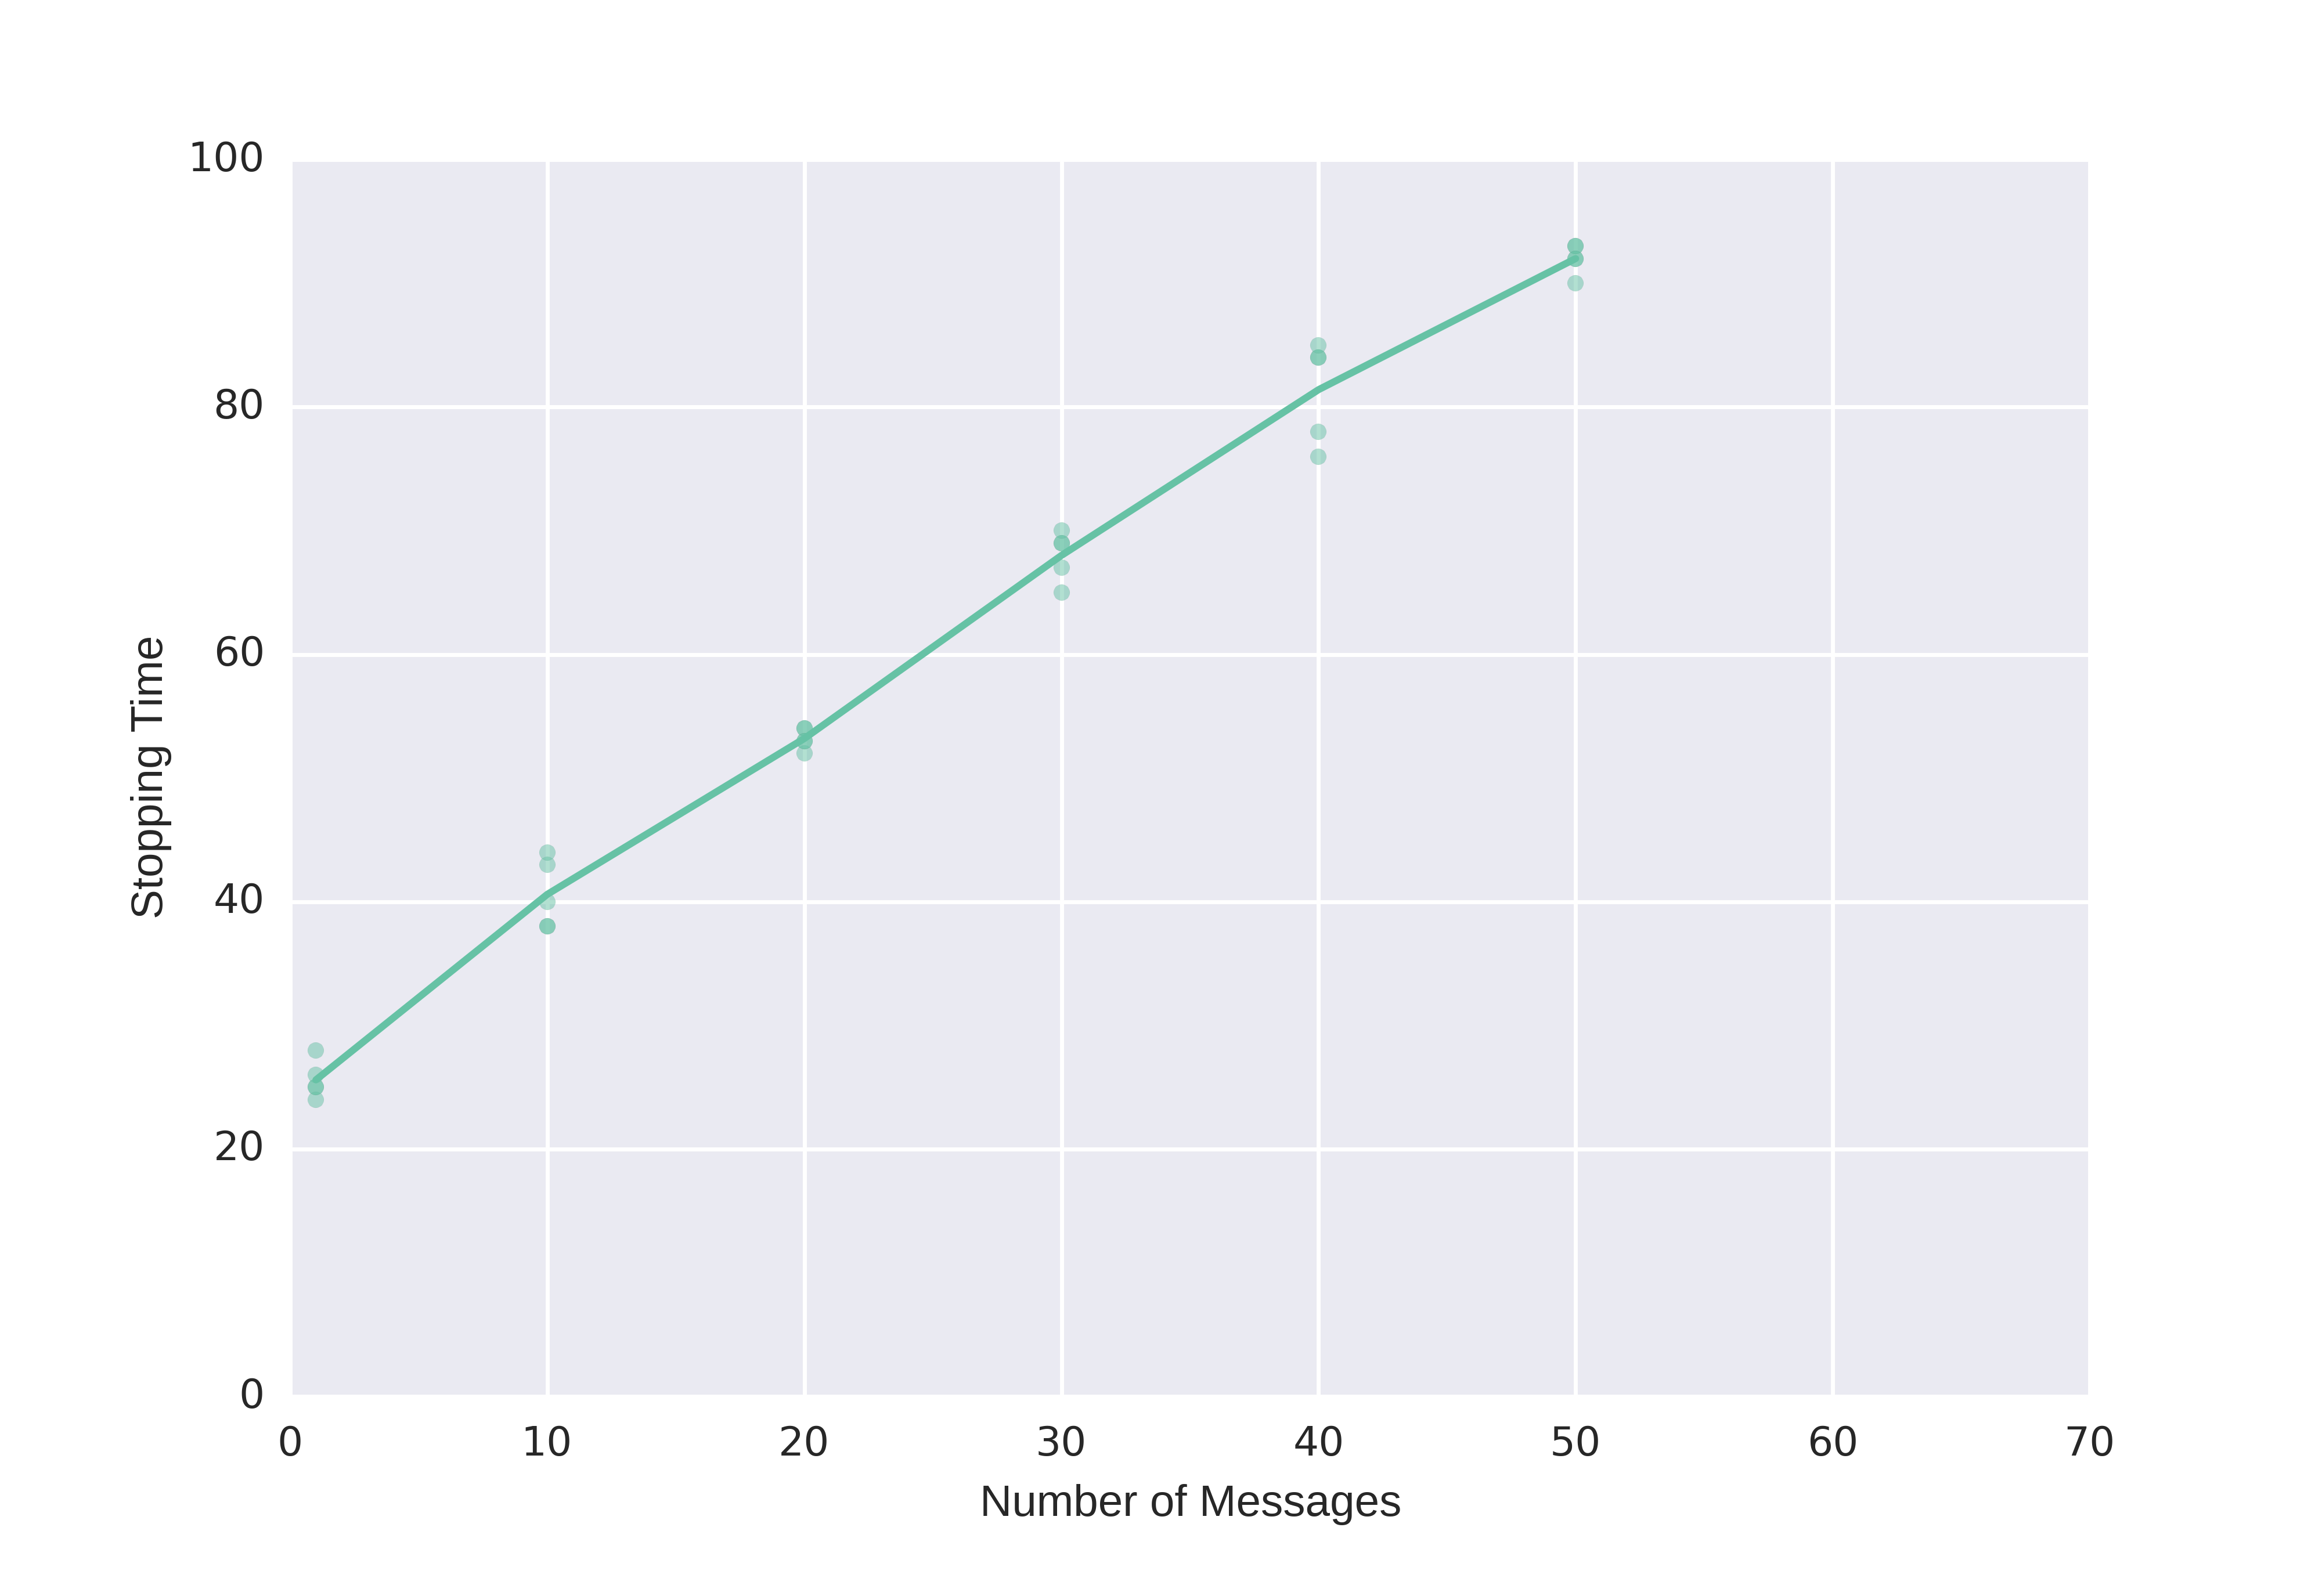
\includegraphics[width=\linewidth]{figures/rlnc-vary-k.png}
\caption{The number of rounds that it takes for the algorithm to terminate is linear in the number in the number of messages}
\label{fig:rlnc-vary-k}
\end{figure} 
\begin{figure}
\centering
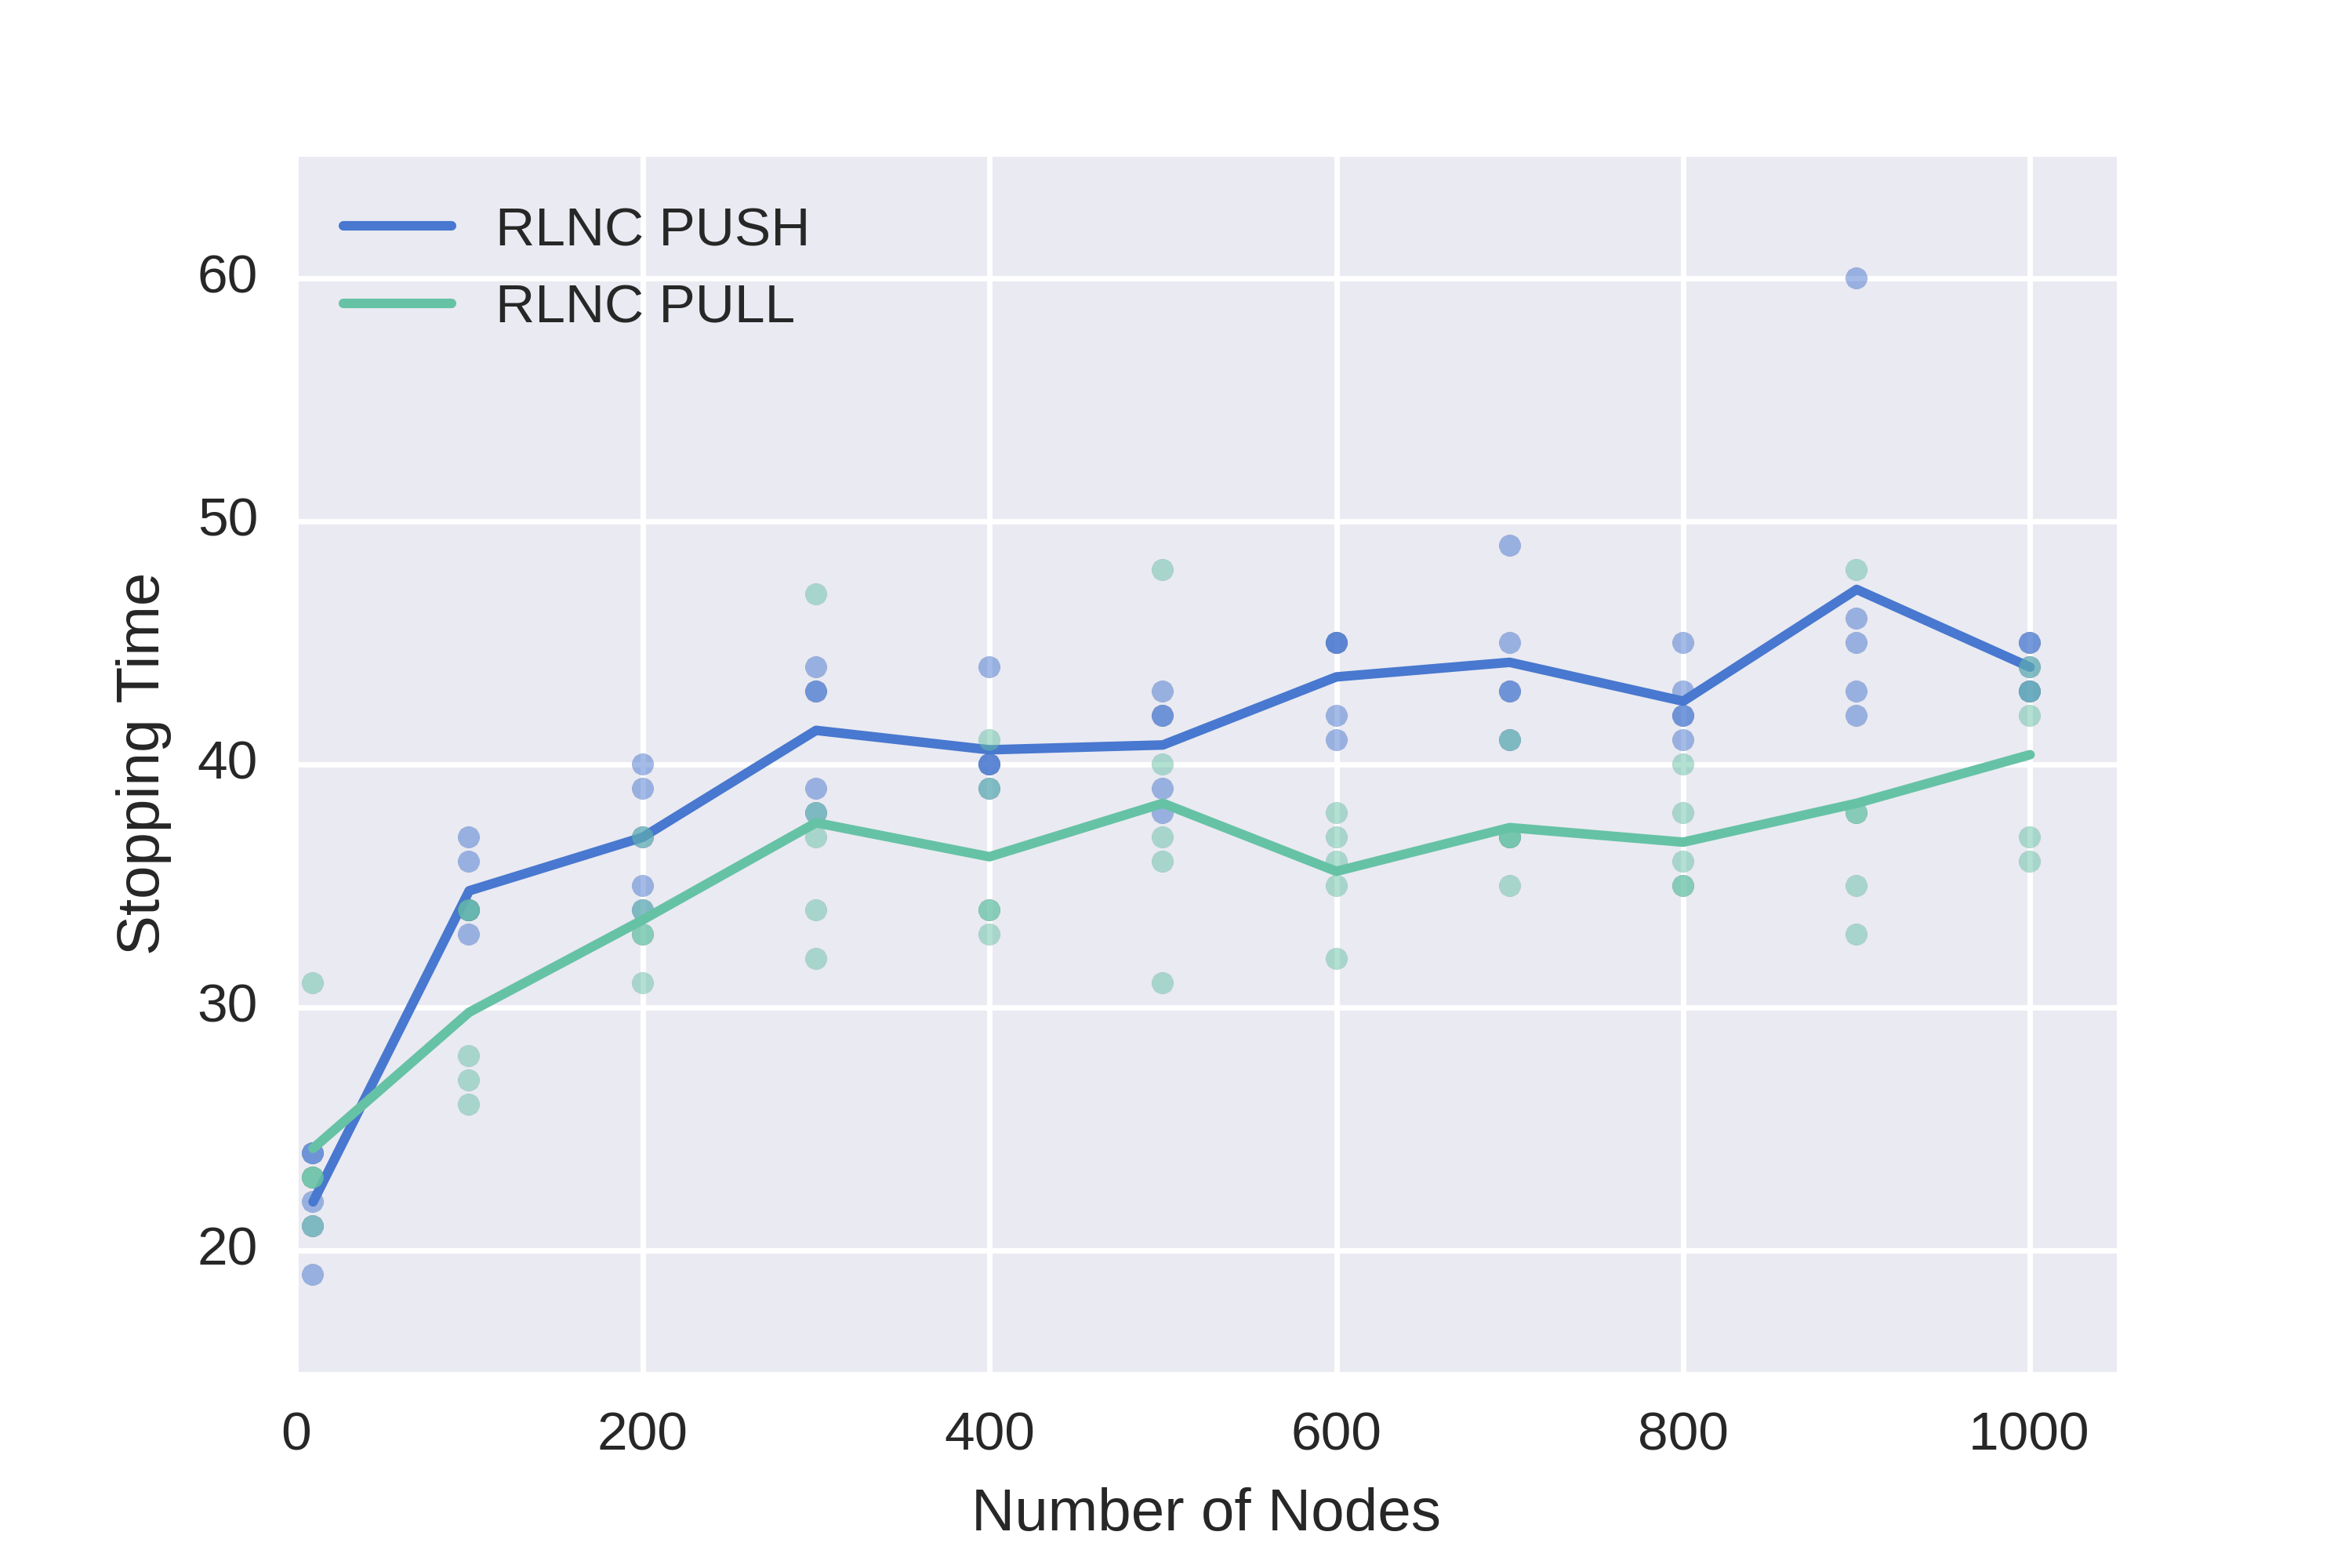
\includegraphics[width=\linewidth]{figures/rlnc-vary-n.png}
\caption{The number of rounds that it takes for the algorithm to terminate is logarithmic in the number of nodes}
\label{fig:rlnc-vary-n}
\end{figure} 


\subsection{Discussion}

\subsection{Conclusions and Future Work}
Code available at \url{https://github.com/newmanne/RLNC-Gossip}.

\nocite{*}
\bibliographystyle{ieeetr}
\bibliography{nips}



%For my project, I plan to read \emph{Analyzing network coding gossip made easy} and \emph{Epidemic algorithms for replicated database maintenance}. I plan to implement the gossip algorithm with RLNC and perform experiments to measure the stopping time. I will investigate the performance on static graphs vs dynamic graphs, on different starting knowledge configurations, and I will investigate the impact of the different ways in which nodes can connect with each other: broadcasting, pushing, pulling, and exchanging. I will compare my results with the theoretical stopping times given in \cite{haeupler2011analyzing}.



\end{document}